\chapter{State of the Art}

\label{ch:State}

\section{Scale of fluctuation}


Due to the complex geological and environmental processes involved, the soil characteristics in situ are rarely homogeneous. The soil characteristics can be highly variable and spatially correlated in the vertical and horizontal directions. As shown in \cref{fig:fig5}, a soil property $g\left ( z \right )$ can be decomposed into a deterministic trend component $t\left ( z \right )$ and a stationary random function $w\left ( z \right )$ as follows: 
\begin{equation}
g\left ( z \right ) = t\left ( z \right ) +  w\left ( z \right ) 
\end{equation}

This concept of the Scale of fluctuation (SoF) was firstly proposed by \cite{vanmarcke1977}, which provides an indicator of the estimated distance over a soil property. It is a convenient measure for describing the spatial variability of a soil property in a random field. A small SoF indicates that the soil oscillates quickly around its mean trend, whereas a large SoF indicates that the property is nearly spatially homogeneous.








For the values of the SoF, scales of fluctuation reported in the literature generally indicate that the horizontal SoF is larger than the vertical SoF. And the range for the vertical SoF is relatively narrow, from 0.06 to 2.6 m, for cone penetration test (CPT) results. However, the range for the horizontal SoF for CPT is fairly broad, from 0.14 to 80 m.




\begin{figure}[!ht]
    \centering
    
    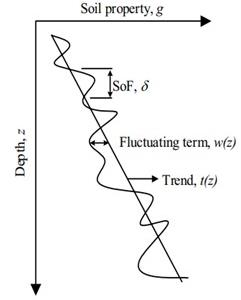
\includegraphics[width = 90mm]{Figures/figure5.jpg}
    \caption{Illustration of the soil inherent variability (follow \cite{nie2015})}
    \label{fig:fig5}
\captionsetup{belowskip=0pt}
\end{figure}



For assessment, in the present study, the autocorrelation fitting method (ACFM) appears to be one of the most widely used methods for estimating SoF. The main idea of ACFM is to fit theoretical models to the sample autocorrelation function $\hat{\rho}\left ( \tau  \right ) $based on an ordinary least squares approach.



Let $\bar{w}$ and $\hat{\sigma}^{2}$ denote the sample mean and the sample variance of $w\left ( z \right )$. where $n\left ( \tau  \right )$denotes the number of pairs that are separated by the distance $\tau$.The sample autocorrelation function can be obtained from the following equation:

\begin{equation}
 \hat{\rho}\left ( \tau  \right ) = \frac{\sum\limits_{i=1}^{n\left ( \tau  \right )}\left [ w\left ( z_{i}  \right )-  \bar{w}  \right ]\left [  w\left ( z_{i} +   \tau \right ) -\bar{w} \right ]   }{\left [ n\left ( \tau  \right )-1 \right ] \hat{\sigma}^{2}  } 
\end{equation}



